\documentclass[xcolor={dvipsnames}]{beamer}

\usepackage[utf8]{inputenc}

\usepackage{times}
\usepackage[frenchb]{babel}

\usepackage{xspace}
\usepackage{graphicx}
\usepackage{amsmath}
\usepackage{amssymb}
\usepackage{amsthm}
\usepackage{latexsym}
\usepackage{lipsum}
\usepackage{tikz}
\usetikzlibrary{positioning}
\usetikzlibrary{automata}
\usepackage{tikz-cd}
\usepackage{mathtools}
\usetikzlibrary{decorations.pathmorphing}

\usetheme{Madrid}

\makeatother
\setbeamertemplate{footline}
{
  \leavevmode%
  \hbox{%
  \begin{beamercolorbox}[wd=.3\paperwidth,ht=2.25ex,dp=1ex,center]{author in head/foot}%
    \usebeamerfont{author in head/foot}\insertshortauthor
  \end{beamercolorbox}%
  \begin{beamercolorbox}[wd=.4\paperwidth,ht=2.25ex,dp=1ex,center]{title in head/foot}%
    \usebeamerfont{title in head/foot}\insertshorttitle\hspace*{3em}
  \end{beamercolorbox}%
  \begin{beamercolorbox}[wd=.3\paperwidth,ht=2.25ex,dp=1ex,right]{author in head/foot}%
    \insertframenumber{} / \inserttotalframenumber\hspace*{1ex}
  \end{beamercolorbox}}%
  \vskip0pt%
}
\makeatletter
\setbeamertemplate{navigation symbols}{}

\AtBeginSection[]{
  \begin{frame}{Sommaire}
  \small \tableofcontents[currentsection, currentsubsection]
  \end{frame} 
}
\AtBeginSubsection[]{
  \begin{frame}{Sommaire}
  \small \tableofcontents[currentsection, currentsubsection]
  \end{frame} 
}

\newcommand\xrsquigarrow[1]{%
  \mathrel{%
    \begin{tikzpicture}[%
      baseline={(current bounding box.south)}
      ]
      \node[%
      ,inner sep=.44ex
      ,align=center
      ] (tmp) {$\scriptstyle #1$};
      \path[%
      ,draw,<-
      ,decorate,decoration={%
        ,zigzag
        ,amplitude=0.7pt
        ,segment length=1.2mm,pre length=3.5pt
      }
      ] 
      (tmp.south east) -- (tmp.south west);
    \end{tikzpicture}
  }
}

\newcommand{\csprogramme}{\textsc{cs}-programme\xspace}
\newcommand{\csprogrammes}{\textsc{cs}-programmes\xspace}
\newcommand{\csclause}{\textsc{cs}-clause\xspace}
\newcommand{\csclauses}{\textsc{cs}-clauses\xspace}

\newcommand{\focusrgb}{0,0,1}
\definecolor{good}{rgb}{0,.7,0}

\definecolor{focusColor}{rgb}{0,0,1}
\definecolor{fig-color-i}{RGB}{ 191, 236, 255}
\definecolor{fig-color2}{RGB}{  144, 221, 255}
\definecolor{fig-color3}{RGB}{  103, 209, 255}
\definecolor{fig-color4}{RGB}{   49, 192, 255}
\definecolor{fig-color-ri}{RGB}{  0, 177, 255}

\author{
  Vivien Pelletier
}
\title[Soutenance de thèse]{Sur-approximations non régulières et\\ terminaison pour l'analyse d'accessibilité}
\date{23 octobre 2017}
\institute
{
  \footnotesize{Encadré par :}\\
  Pierre Réty et Yohan Boichut
}
\titlegraphic{
  \begin{tabular}{p{0.4\textwidth} p{0.3\textwidth}p{0.25\textwidth}}
    \vspace{0pt} 
\includegraphics[width=0.2\textwidth]{media/logos/lifo.png} & & \vspace{4pt} 
\includegraphics[width=0.2\textwidth]{media/logos/univ.png}
  \end{tabular}
}

\begin{document}

\maketitle

\section{Introduction}

\begin{frame}{Systèmes complexes}
  \begin{block}{Système complexe}
    Un système complexe est un ensemble constitué d'un grand nombre d'entités en interaction qui empêchent l'observateur de prévoir sa rétroaction, son comportement ou évolution par le calcul.
  \end{block}
  \pause
  \begin{exampleblock}{Systèmes complexes}
    \begin{itemize}
    \item programmes informatiques,
    \item protocoles de sécurité,
    \item circuits logiques \ldots
    \end{itemize}
  \end{exampleblock}
\end{frame}

\begin{frame}{Le génie logiciel}
  \begin{columns}
    \begin{column}{0.6\textwidth}
      \begin{center}
        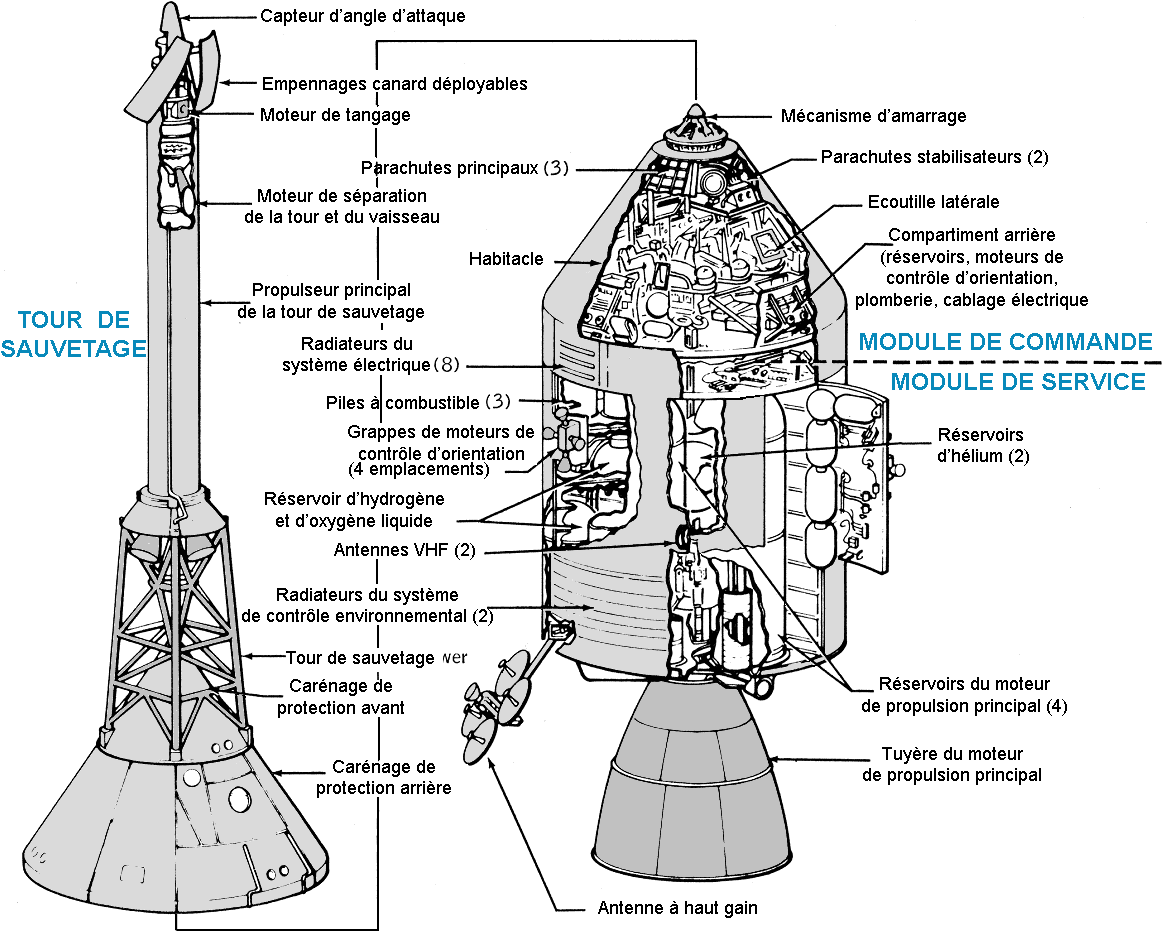
\includegraphics[height=4cm]{media/apollo.png}
      \end{center}
      \onslide<2>
      \begin{block}{Génie logiciel}
        L'ensemble des activités de conception et de mise en œuvre des produits et des procédures tendant à rationaliser la production du logiciel et son suivi.
      \end{block}
    \end{column}
    \begin{column}{0.4\textwidth}
      \onslide<1->
      \begin{center}
        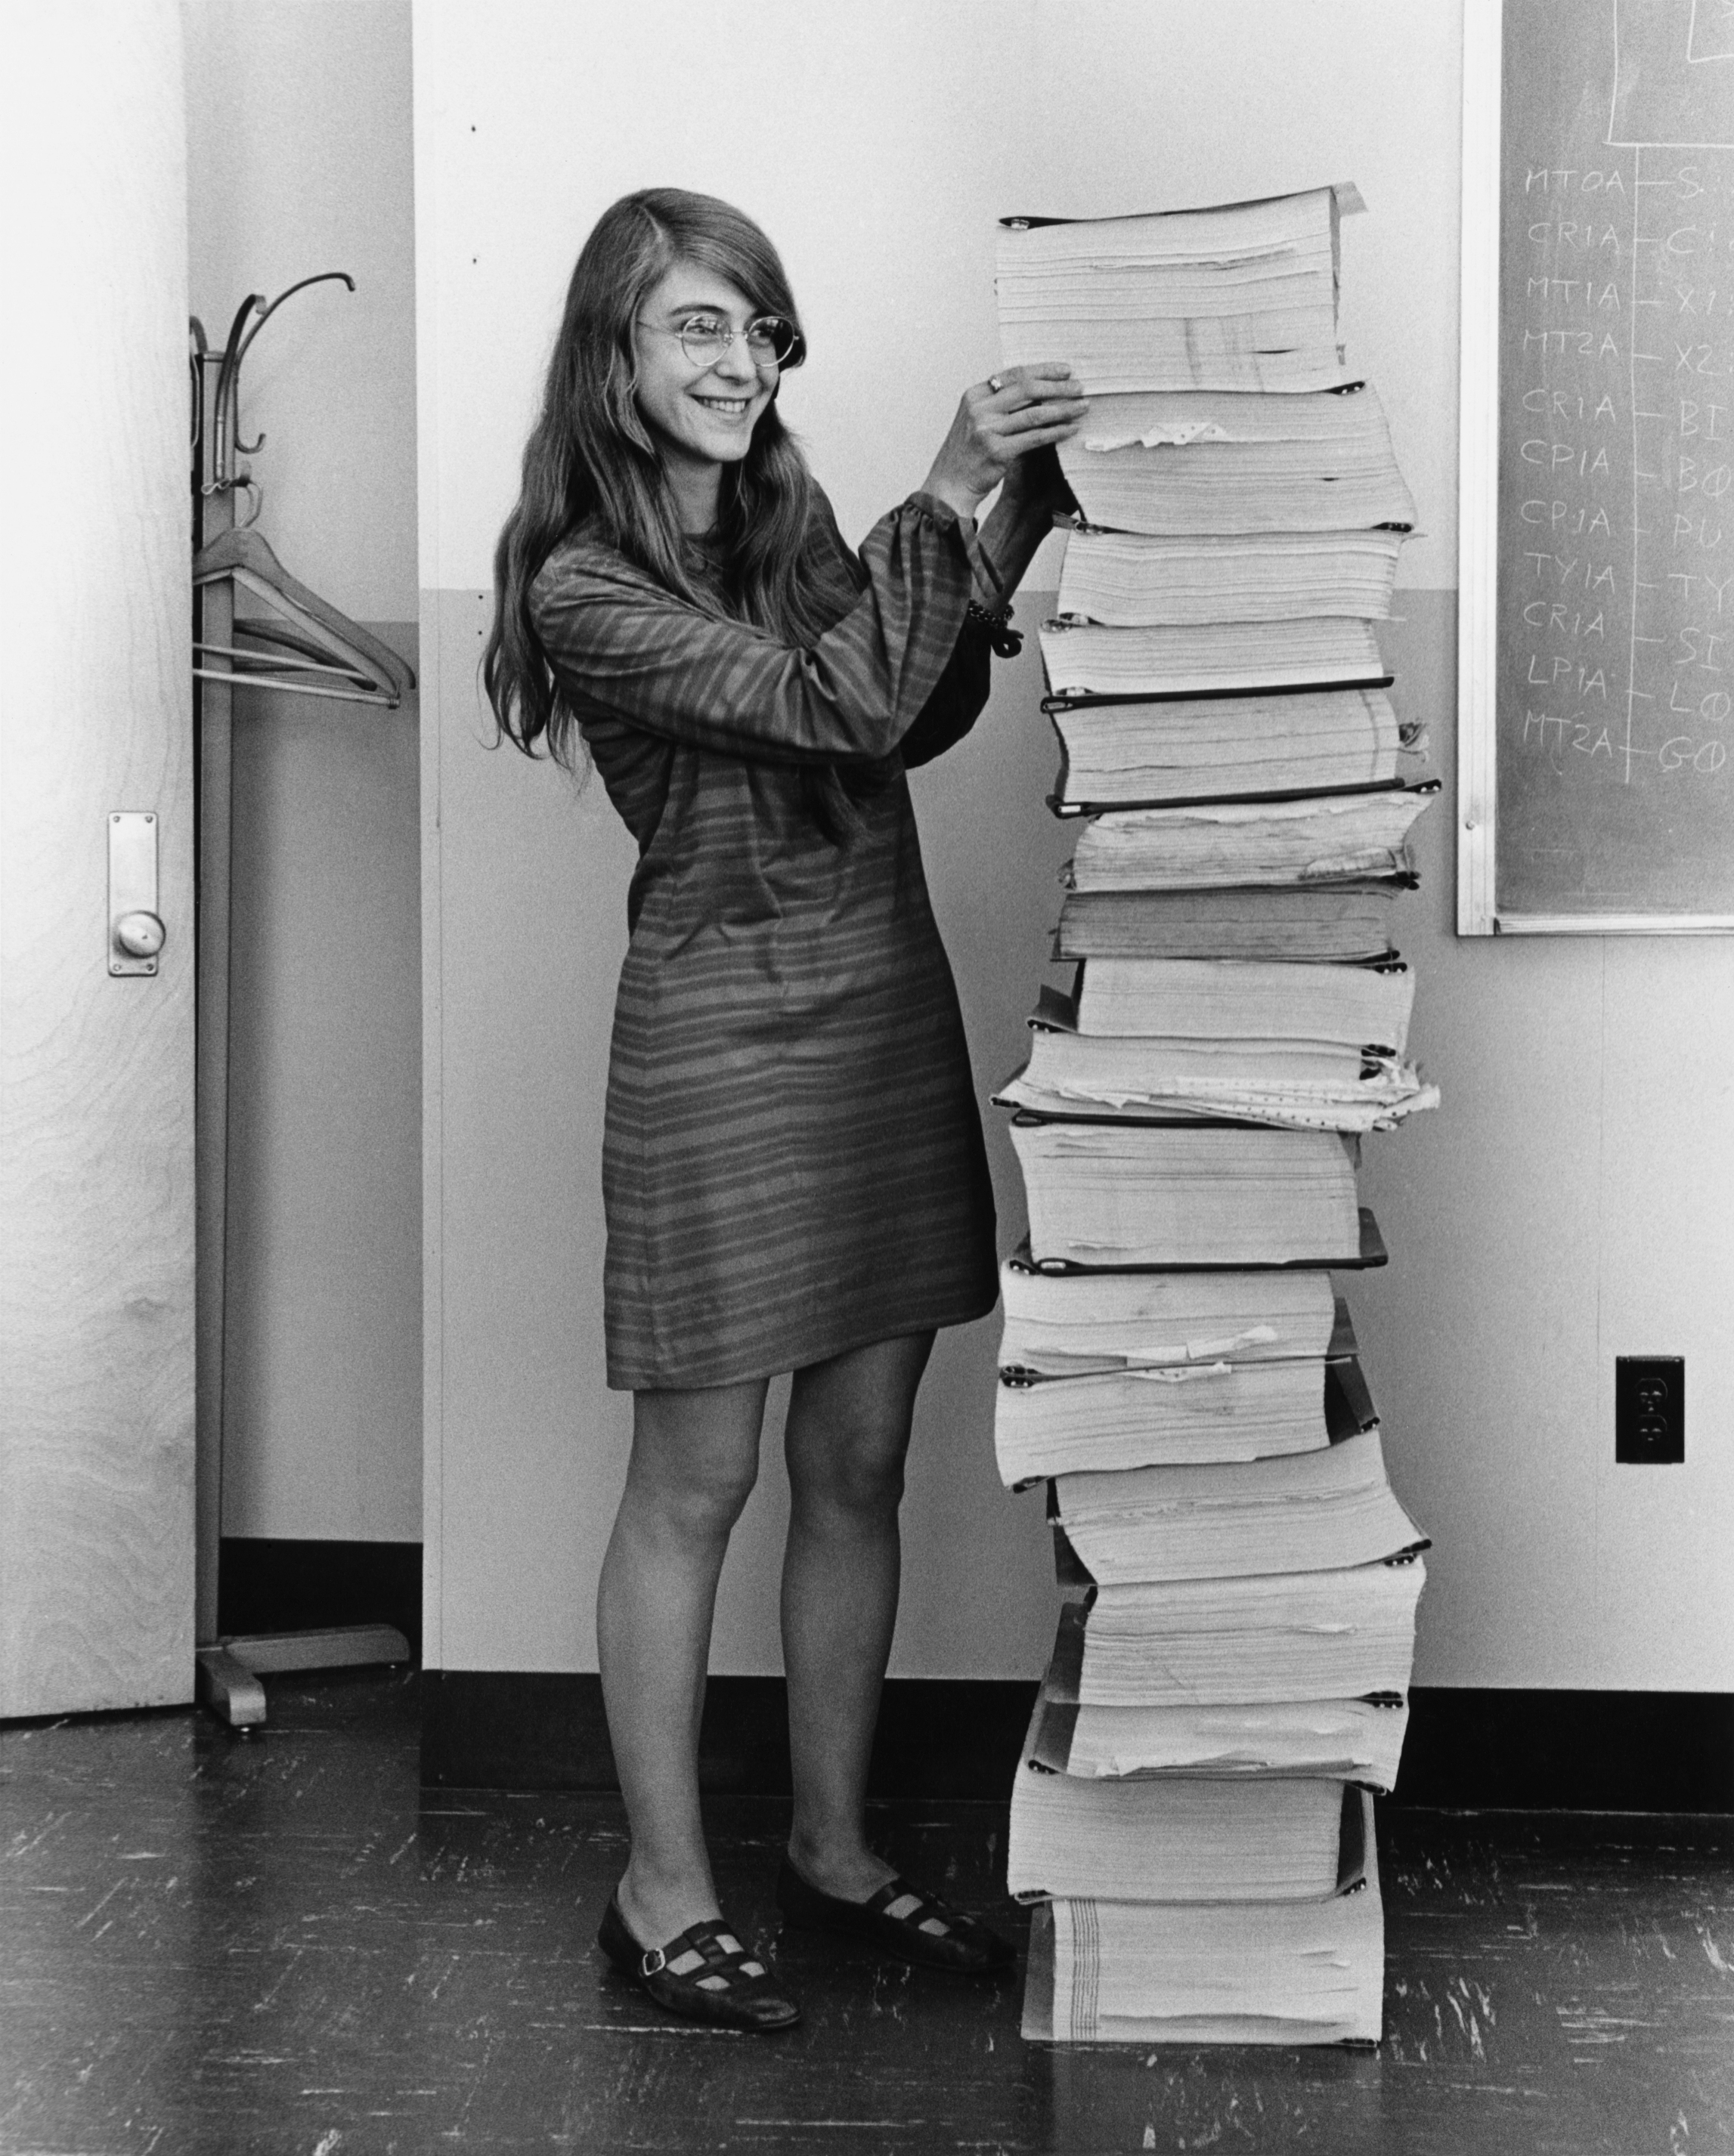
\includegraphics[width=0.9\textwidth]{media/MHamilton.jpg}
      \end{center}
    \end{column}
  \end{columns}
\end{frame}

\begin{frame}{Vérification}
  Conformité et fiabilité d'un système complexe ?
  \begin{block}{}
    \begin{itemize}[<+->]
    \item Les tests
      \begin{itemize}
      \item si l'ensemble d'entrées est trop grand ou infini ?
      \end{itemize}
    \item Les méthodes formelles
      \begin{itemize}
      \item analyse statique par interprétation abstraite
      \item vérification déductive
      \item vérification de modèles
      \end{itemize}
    \end{itemize}
  \end{block}
\end{frame}

\begin{frame}{Analyse statique par interprétation abstraite}
  \begin{columns}
    \begin{column}{0.3\textwidth}
      \begin{center}
        
\includegraphics[width=0.5\textwidth]{media/fichier.png}
        
\includegraphics[width=\textwidth]{media/entonnoir.png}
        
\includegraphics[width=0.25\textwidth]{media/fichier.png}
      \end{center}
    \end{column}
    \begin{column}{0.5\textwidth}
      \begin{block}{}
        \begin{itemize}
        \item Constat
          \begin{itemize}
          \item trop d'informations
          \end{itemize}
        \item Solution
          \begin{itemize}
          \item utilisation d'abstractions
          \end{itemize}
        \item Difficulté
          \begin{itemize}
          \item garder suffisamment d'informations
          \item mais pas trop
          \end{itemize}
        \end{itemize}
      \end{block}
    \end{column}
  \end{columns}
\end{frame}

\begin{frame}{Vérification déductive}
  \begin{overprint}
    \onslide<1>
    \begin{tikzpicture}
      \node (shredder) at (0,1.5) {
\includegraphics[width=0.3\textwidth]{media/shredder.png}};
    \end{tikzpicture}
    \onslide<2>
    \begin{tikzpicture}
      \node (shredder) at (0,1.5) {
\includegraphics[width=0.3\textwidth]{media/shredder.png}};
      \node[circle, minimum size=0.5cm, very thick, fill=white, draw] (small) at (0,0.4) {};
      \node[circle, minimum size=7cm, very thick, draw] (big) at (6,-0.5) {};
      
      \node[minimum width=1.7cm, minimum height=1cm, draw] (dom3pre) at (6, -2) {\tiny{préconditions}};
      \node[minimum width=1.7cm, minimum height=1cm, below=0 of dom3pre, draw] (dom3post) {\tiny{postconditions}};
      
      \draw[very thick] (small) -- (big);
    \end{tikzpicture}
    \onslide<3>
    \begin{tikzpicture}
      \node (shredder) at (0,1.5) {
\includegraphics[width=0.3\textwidth]{media/shredder.png}};
      \node[circle, minimum size=0.5cm, very thick, fill=white, draw] (small) at (0,0.4) {};
      \node[circle, minimum size=7cm, very thick, draw] (big) at (6,-0.5) {};
      
      \node[minimum width=1.7cm, minimum height=1cm, draw] (dom1pre) at (4.75, 1.25) {\tiny{préconditions}};
      \node[minimum width=1.7cm, minimum height=1cm, below=0 of dom1pre, draw] (dom1post) {\tiny{postconditions}};
      
      \node[minimum width=1.7cm, minimum height=1cm, draw] (dom2pre) at (7.25, 1.25) {\tiny{préconditions}};
      \node[minimum width=1.7cm, minimum height=1cm, below=0 of dom2pre, draw] (dom2post) {\tiny{postconditions}};
      
      \node[minimum width=1.7cm, minimum height=1cm, draw] (dom3pre) at (6, -2) {\tiny{préconditions}};
      \node[minimum width=1.7cm, minimum height=1cm, below=0 of dom3pre, draw] (dom3post) {\tiny{postconditions}};
      
      \draw[very thick] (small) -- (big);
      
      \draw[->, thick] (dom1post.south) |- (5.5,-0.75) -- (dom3pre.134);
      \draw[->, thick] (dom2post.-134) |- (6.5,-0.75) -- (dom3pre.46);
      \draw[->, thick] (dom2post.-46) |- (8.25,-0.75) -- (8.25,2) -| (dom2pre.46);

      \draw[->, thick] (big.66) -| (dom2pre.134);
      \draw[->, thick] (big.north) -- (6,2.5 ) -| (dom1pre.north);
    \end{tikzpicture}
  \end{overprint}
\end{frame}

\begin{frame}{Vérification de modèles}
  \begin{block}{}
    \begin{itemize}
    \item Analyse exhaustive
    \item Représentation astucieuse
    \end{itemize}
  \end{block}
  \begin{columns}
    \begin{column}{0.5\textwidth}
      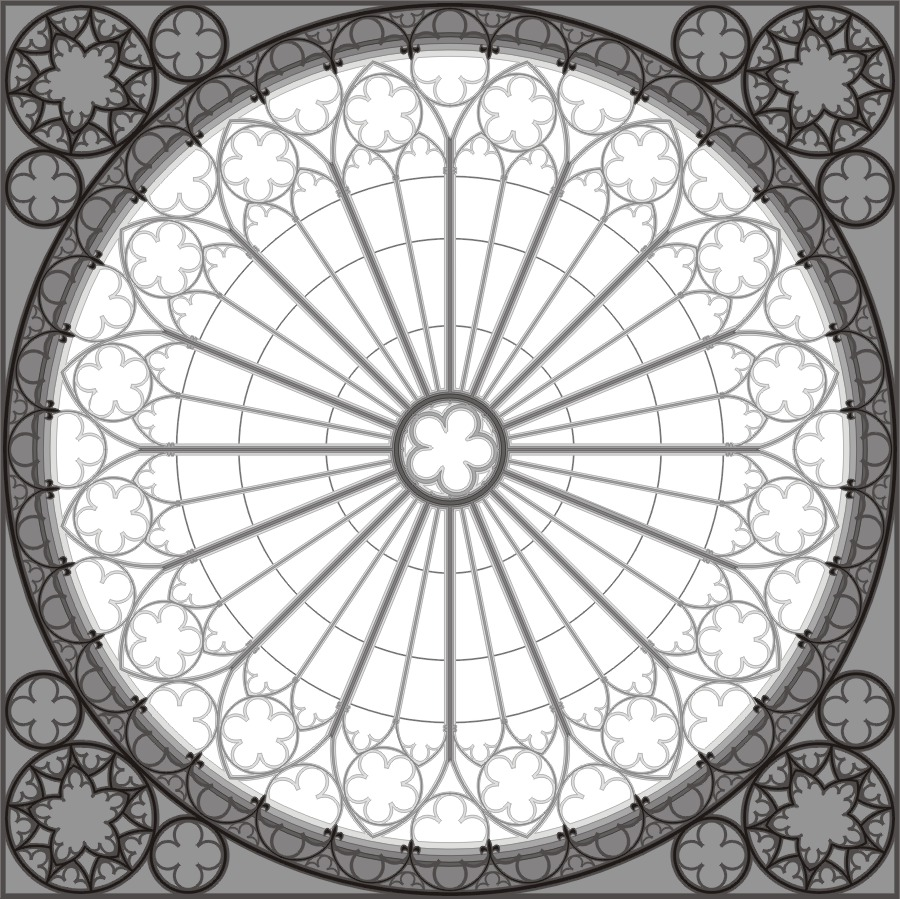
\includegraphics[width=\textwidth]{media/rosace.jpg}
    \end{column}
    \begin{column}{0.5\textwidth}
      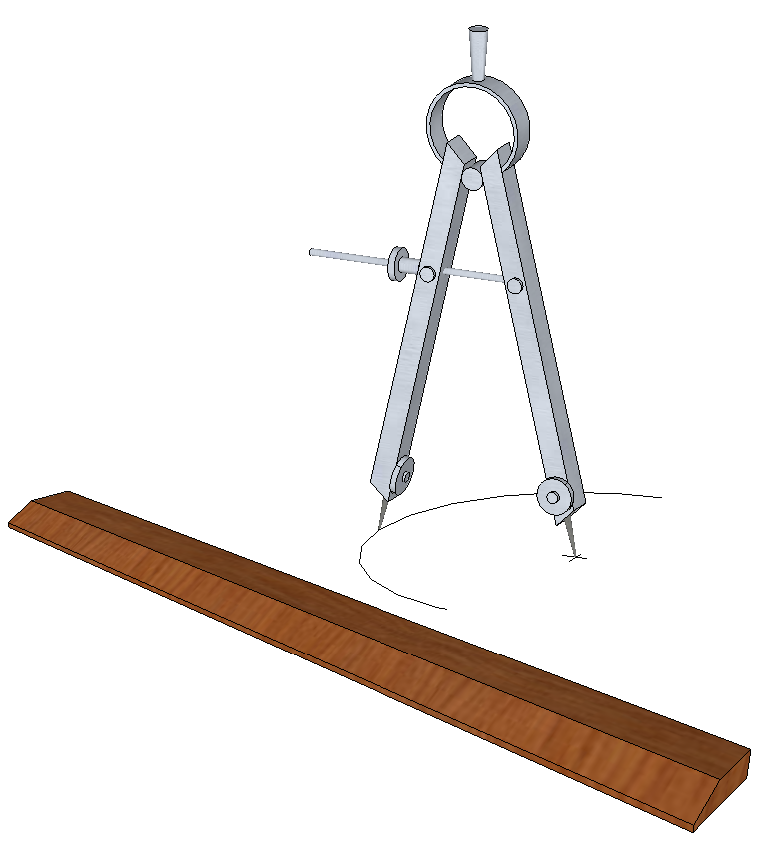
\includegraphics[width=\textwidth]{media/compass_ruler.png}
    \end{column}
  \end{columns}
\end{frame}

\begin{frame}{Analyse d'accessibilité}
  Configurations
  \begin{block}{}
    \begin{itemize}[<+->]
    \item Ensemble des configurations accessibles
    \item Ensemble des configurations indésirables
    \end{itemize}
  \end{block}
  \begin{columns}
    \begin{column}{0.45\textwidth}
      \onslide<3->
      \begin{center}
        \begin{tikzpicture}
          \draw[fill=ProcessBlue, fill opacity=0.5] (0,0) ellipse (1 and 0.75);
          \node (r*i) at (0,0) {\scriptsize{Accessibles}};
          \draw[fill=Red, fill opacity=0.5] (1.75,0) ellipse (1 and 0.75);
          \node (bad) at (1.75,0) {\scriptsize{Indésirables}};
        \end{tikzpicture}\\
        Il existe une configuration\\ indésirable accessible
      \end{center}
    \end{column}
    \begin{column}{0.45\textwidth}
      \onslide<4>
      \begin{center}
        \begin{tikzpicture}
          \draw[fill=ProcessBlue, fill opacity=0.5] (0,0) ellipse (1 and 0.75);
          \node (r*i) at (0,0) {\scriptsize{Accessibles}};
          \draw[fill=Red, fill opacity=0.5] (2.5,0) ellipse (1 and 0.75);
          \node (bad) at (2.5,0) {\scriptsize{Indésirables}};
        \end{tikzpicture}\\
        Aucune configuration indésirable\\ n'est accessible
      \end{center}
    \end{column}
  \end{columns}
\end{frame}

\begin{frame}{Calcul de l'ensemble des configurations accessibles}
  \begin{itemize}[<+->]
  \item Configurations initiales : $I$
  \item Dynamique : $R$
  \end{itemize}
  \begin{center}
    \begin{tikzpicture}
      \onslide<7->
      \draw[fill=fig-color-ri] (4,0) ellipse (5 and 2.2);
      \node (r*i) at (7.75,0) {$R^*(I)$};

      \onslide<6->
      \draw[fill=fig-color4] (3,0) ellipse (4 and 1.9);
      \node (...) at (5.75,0) {$\cdots$};
      
      \onslide<5->
      \draw[fill=fig-color3] (2,0) ellipse (3 and 1.6);
      \node (r2i) at (3.75,0) {$R^2(I)$};

      \onslide<4->      
      \draw[fill=fig-color2] (1,0) ellipse (2 and 1.3);
      \node (ri) at (1.75,0) {$R(I)$};

      \onslide<3->
      \draw[fill=fig-color-i] (0,0) ellipse (1 and 1);
      \node (i) at (0,0) {$I$};
      
      \onslide<1->
    \end{tikzpicture}
  \end{center}
\end{frame}

\begin{frame}{Sur-approximations}
  \begin{center}
    \begin{tikzpicture}
      \draw[fill=Goldenrod, fill opacity=0.5] (0,0) ellipse (2 and 1);
      \node (r*i) at (-1.25,0) {$\mathcal H$};
      
      \draw[fill=ProcessBlue, fill opacity=0.5] (0,0) ellipse (1 and 0.75);
      \node (r*i) at (0,0) {\scriptsize{Accessibles}};
      \draw[fill=Red, fill opacity=0.5] (3.5,0) ellipse (1 and 0.75);
      \node (bad) at (3.5,0) {\scriptsize{Indésirables}};
    \end{tikzpicture}\\
    Aucune configuration indésirable accessible\\
  \end{center}
  \begin{columns}
    \begin{column}{0.5\textwidth}
      \pause
      \begin{center}
        \begin{tikzpicture}
          \draw[fill=Goldenrod, fill opacity=0.5] (0,0) ellipse (2 and 1);
          \node (r*i) at (-1.25,0) {$\mathcal H$};
          
          \draw[fill=ProcessBlue, fill opacity=0.5] (0,0) ellipse (1 and 0.75);
          \node (r*i) at (0,0) {\scriptsize{Accessibles}};
          \draw[fill=Red, fill opacity=0.5] (1.75,0) ellipse (1 and 0.75);
          \node (bad) at (1.75,0) {\scriptsize{Indésirables}};
        \end{tikzpicture}\\
        Il existe une configuration\\ indésirable accessible
      \end{center}
    \end{column}
    \begin{column}{0.5\textwidth}
      \pause
      \begin{center}
        \begin{tikzpicture}
          \draw[fill=Goldenrod, fill opacity=0.5] (0,0) ellipse (2 and 1);
          \node (r*i) at (-1.25,0) {$\mathcal H$};
          
          \draw[fill=ProcessBlue, fill opacity=0.5] (0,0) ellipse (1 and 0.75);
          \node (r*i) at (0,0) {\scriptsize{Accessibles}};
          \draw[fill=Red, fill opacity=0.5] (2.5,0) ellipse (1 and 0.75);
          \node (bad) at (2.5,0) {\scriptsize{Indésirables}};
        \end{tikzpicture}\\
        Aucune configuration \\indésirable accessible,\\ c'est un faux-positif
      \end{center}
    \end{column}
  \end{columns}
\end{frame}

\begin{frame}{Notre modélisation}
  \begin{block}{}
    \begin{itemize}[<+->]
    \item Configuration : un terme
    \item Configurations initiales : un langage de termes
    \item Dynamique du système : un système de réécriture
    \item Configurations indésirables : un langage de termes
    \end{itemize}
  \end{block}
\end{frame}

\section{Préliminaires}

\begin{frame}{Les termes}
  \begin{columns}
    \begin{column}{0.65\textwidth}
      \begin{block}{}
        \begin{itemize}[<+->]
        \item Des symboles d'arité fixe : $f^{\backslash 2}$
        \item Un alphabet : $\{ a^{\backslash 0}, b^{\backslash 0}, s^{\backslash 1}, h^{\backslash 1}, f^{\backslash 2}\}$
        \item Un terme : $f(f(s(a), a),s(f(b,b)))$
        \end{itemize}
      \end{block}
    \end{column}
    \begin{column}{0.35\textwidth}
      \onslide<4>
      \begin{tikz}
        \node {$f$}
          child { node {$f$}
            child { node {$s$}
              child { node {$a$} } }
            child { node {$a$} } }
          child { node {$s$}
            child {node {$f$}
              child { node {$b$} }
              child { node {$b$} } } };
      \end{tikz}
    \end{column}
  \end{columns}
\end{frame}

\begin{frame}{Langages formels}
  Un ensemble de termes
  \begin{block}{}
    \begin{itemize}[<+->]
    \item Langages réguliers : $\{f(s^*(a),s^*(a))\}$
    \item Langages synchronisés : $\{f(s^n(a),s^n(a)) \mid n \geq 0\}$
    \item Langages algébriques : $\{s^n(h^n(a)) \mid n \geq 0\}$
    \item Langages synchronisés algébriques : $\{f(s^n(h^n(a)),s^n(h^n(b))) \mid n \geq 0\}$
    \end{itemize}
  \end{block}
  \begin{overprint}
    \onslide<1>
    \begin{tikzpicture}
      \node[shape=rectangle, draw] (reg) at (0,0) {\scriptsize{Réguliers}};
    \end{tikzpicture}
    \onslide<2>
    \begin{tikzpicture}
      \node[shape=rectangle, draw] (reg) at (0,0) {\scriptsize{Réguliers}};
      \node[shape=rectangle, draw] (synch) at (3,1) {\scriptsize{Synchronisés}};
      
      \draw[->] (reg.east) -- (synch.west);
    \end{tikzpicture}
    \onslide<3>
    \begin{tikzpicture}
      \node[shape=rectangle, draw] (reg) at (0,0) {\scriptsize{Réguliers}};
      \node[shape=rectangle, draw] (synch) at (3,1) {\scriptsize{Synchronisés}};
      \node[shape=rectangle, draw] (algeio) at (3,0) {\scriptsize{Algébriques IO}};
      \node[shape=rectangle, draw] (algeoi) at (3,-1) {\scriptsize{Algébriques OI}};
      
      \draw[->] (reg.east) -- (synch.west);
      \draw[->] (reg.east) -- (algeio.west);
      \draw[->] (reg.east) -- (algeoi.west);
    \end{tikzpicture}
    \onslide<4>
    \begin{tikzpicture}
      \node[shape=rectangle, draw] (reg) at (0,0) {\scriptsize{Réguliers}};
      \node[shape=rectangle, draw] (synch) at (3,1) {\scriptsize{Synchronisés}};
      \node[shape=rectangle, draw] (algeio) at (3,0) {\scriptsize{Algébriques IO}};
      \node[shape=rectangle, draw] (algeoi) at (3,-1) {\scriptsize{Algébriques OI}};
      \node[shape=rectangle, draw] (synchalge) at (7,1) {\scriptsize{Synchronisés Algébriques}};
      
      \draw[->] (reg.east) -- (synch.west);
      \draw[->] (reg.east) -- (algeio.west);
      \draw[->] (reg.east) -- (algeoi.west);
      \draw[->] (synch.east) -- (synchalge.west);
      \draw[->] (algeio.east) -- (synchalge.west);
    \end{tikzpicture}
  \end{overprint}
\end{frame}

\begin{frame}{Variables}
  \begin{columns}
    \begin{column}{0.6\textwidth}
      \begin{itemize}
      \item<1-> Ensemble de variables : $\mathcal X = \{x, y\}$
      \item<2-> La substitution : $\sigma = (x / s(b))$
      \item<4-> Le filtrage : $\sigma(t) = t'$
      \item<6-> L'unification : $\alpha(t) = \alpha(t')$
      \end{itemize}
    \end{column}
    \begin{column}{0.4\textwidth}
      \begin{overprint}
        \onslide<2-3>
        \begin{center}
          $t = f(x,s(a))$\\
          \begin{tikzpicture}[level distance = 1cm]
            \node {$f$}
            child { node {$x$}}
            child { node {$s$}
              child {node {$a$}}};
          \end{tikzpicture}
        \end{center}
        \onslide<4-5>
        \begin{center}
          $t = f(x,s(a))$\\
          \begin{tikzpicture}[level distance = 1cm]
            \node {$f$}
            child { node {$x$}}
            child { node {$s$}
              child {node {$a$}}};
          \end{tikzpicture}
        \end{center}
        \onslide<6->
        \begin{center}
          \begin{columns}
            \begin{column}{0.5\textwidth}
              $t = f(x,s(a))$\\
              \begin{tikzpicture}[level distance = 1cm]
                \node {$f$}
                child { node {$x$}}
                child { node {$s$}
                  child {node {$a$}}};
              \end{tikzpicture}
            \end{column}
            \begin{column}{0.5\textwidth}
              $t' = f(s(b),y)$\\
              \begin{tikzpicture}[level distance = 1cm]
                \node {$f$}
                child { node {$s$}
                  child {node {$b$}}}
                child { node {$y$}};
              \end{tikzpicture}
            \end{column}
          \end{columns}
        \end{center}
      \end{overprint}
      
      \begin{overprint}
        \onslide<3>
        \begin{center}
          $\sigma(t) = f(s(b),s(a))$\\
          \begin{tikzpicture}[level distance = 1cm]
            \node {$f$}
            child { node {$s$}
              child {node {$b$}}}
            child { node {$s$}
              child {node {$a$}}};
          \end{tikzpicture}
        \end{center}
        \onslide<5>
        \begin{center}
          $t' = f(s(b),s(a))$\\
          \begin{tikzpicture}[level distance = 1cm]
            \node {$f$}
            child { node {$s$}
              child {node {$b$}}}
            child { node {$s$}
              child {node {$a$}}};
          \end{tikzpicture}
        \end{center}
        \onslide<7>
        \begin{center}
          $\alpha(t) = \alpha(t') = f(s(b),s(a))$\\
          $\alpha = (x/s(b), y/s(a))$\\
          \begin{tikzpicture}[level distance = 1cm]
            \node {$f$}
            child { node {$s$}
              child {node {$b$}}}
            child { node {$s$}
              child {node {$a$}}};
          \end{tikzpicture}
        \end{center}
      \end{overprint}
    \end{column}
  \end{columns}
\end{frame}

\begin{frame}{Systèmes de réécriture}
  \begin{itemize}
  \item $r$ et $l$ des termes
  \item $Var(r) \subseteq Var(l)$
  \item $l \rightarrow r$ est une règle de réécriture
  \end{itemize}
  \begin{center}
    $s(x) \rightarrow s(s(x))$\\
    $t = f(y,s(a))$\\
    \onslide<2->
    $\sigma(s(x)) = s(a)$ avec $\sigma = (x / a)$\\
    \onslide<3->
    $t \rightarrow t'$ \\
    \onslide<5>
    $t' = f(y,s(s(a)))$ \\
    \onslide<1->
    \begin{overprint}
      \onslide<1-3>
      \begin{center}
        \begin{tikzpicture}[level distance = 1cm]
          \node {$f$}
          child { node {$b$}}
          child { node {$s$}
            child {node {$a$}}};
        \end{tikzpicture}
      \end{center}
      \onslide<4>
      \begin{center}
        \begin{tikzpicture}[level distance = 1cm]
          \node {$f$}
          child { node {$b$}}
          child { node {$s$}
            child { node {$s$}
              child {node {$x$}}}};
        \end{tikzpicture}
      \end{center}
      \onslide<5>
      \begin{center}
        \begin{tikzpicture}[level distance = 1cm]
          \node {$f$}
          child { node {$b$}}
          child { node {$s$}
            child { node {$s$}
              child {node {$a$}}}};
        \end{tikzpicture}
      \end{center}
    \end{overprint}
  \end{center}
\end{frame}

\section{Sur-approximations d'ensembles de descendants}

\begin{frame}{Les différentes techniques}
  \begin{tikzpicture}[every node/.append style={shape=rectangle, draw}]

    % define style for focused node
    \tikzstyle{focus} = [focusColor, thick]
    \tikzstyle{focusRed} = [red, thick]

    % define command for each node for overprinted color
    \newcommand*\nodeStyleReg{}
    \newcommand*\nodeStyleSync{}
    \newcommand*\nodeStyleAlge{}
    \newcommand*\nodeStyleSAlge{}

    % Associate color to slide pause number
    \only<1-2>{ \renewcommand*\nodeStyleReg{focus} }
    \only<3>{ \renewcommand*\nodeStyleAlge{focus} }
    \only<4>{ \renewcommand*\nodeStyleSync{focus} }
    \only<5>{ \renewcommand*\nodeStyleSAlge{focus} }
    \only<6>{ \renewcommand*\nodeStyleSync{focusRed} }

    % Create node for each language class
    \node[\nodeStyleReg] (reg) at (0,0) {\scriptsize{Réguliers}};
    \node[\nodeStyleSync] (synch) at (3,1) {\scriptsize{Synchronisés}};
    \node[\nodeStyleAlge] (algeio) at (3,0) {\scriptsize{Algébriques IO}};
    \node[\nodeStyleAlge] (algeoi) at (3,-1) {\scriptsize{Algébriques OI}};
    \node[\nodeStyleSAlge] (synchalge) at (7,1) {\scriptsize{Synchronisés Algébriques}};

    % Link nodes to show class inclusions
    \draw[->] (reg.east) -- (synch.west);
    \draw[->] (reg.east) -- (algeio.west);
    \draw[->] (reg.east) -- (algeoi.west);
    \draw[->] (synch.east) -- (synchalge.west);
    \draw[->] (algeio.east) -- (synchalge.west);
  \end{tikzpicture}
  \vspace{\baselineskip}
  \begin{overprint}
    \onslide<1>
    \begin{itemize}
    \item RTA, 1998, T. Genet, {\footnotesize Decidable approximations of sets of descendants and sets of normal forms}
    \item CADE, 2000, T. Genet et F. Klay, {\footnotesize Rewriting for cryptographic protocol verification}
    \item JSC, 2010, T. Genet et V. Rusu, {\footnotesize Equational approximations for tree automata completion}
    \end{itemize}
    \onslide<2>
    \begin{itemize}
    \item IPL, 2008, Y. Boichut et P.-C. Héam, {\footnotesize A theoretical limit for safety verification techniques with regular fix-point computations}
    \end{itemize}
    \onslide<3>
    \begin{itemize}
    \item RTA, 2011, J. Kochems et L. Ong, {\footnotesize Improved functional flow and reachability analyses using indexed linear tree grammars}
    \end{itemize}
    \onslide<4>
    \begin{itemize}
    \item RTA, 2013, Y. Boichut, J. Chabin, et P. Réty, {\footnotesize Over-approximating descendants by synchronized tree languages}
    \end{itemize}
    \onslide<5>
    \begin{itemize}
    \item LATA, 2015, Y. Boichut, J. Chabin, et P. Réty, {\footnotesize Towards more precise rewriting approximations}
    \end{itemize}
    \onslide<6>
    \begin{itemize}
    \item WRLA, 2016, Y. Boichut, V. Pelletier, et P. Réty, {\footnotesize Synchronized tree languages for reachability in non-right-linear term rewrite systems}
    \end{itemize}
  \end{overprint}
\end{frame}

\subsection{Méthode de complétion}

\begin{frame}{Méthode de complétion}
  \begin{center}
    \begin{tikzpicture}
      \onslide<5->
      \draw[fill=fig-color-ri] (4,0) ellipse (5 and 2.2);
      \node (r*i) at (7.75,0) {$Prog'$};

      \onslide<4->
      \draw[fill=fig-color4] (3,0) ellipse (4 and 1.9);
      \node (...) at (5.75,0) {$\cdots$};
      
      \onslide<3->
      \draw[fill=fig-color3] (2,0) ellipse (3 and 1.6);
      \node (r2i) at (4,0) {$R^2(Prog)$};

      \onslide<2->      
      \draw[fill=fig-color2] (1,0) ellipse (2 and 1.3);
      \node (ri) at (1.75,0) {$R(Prog)$};

      \onslide<1->
      \draw[fill=fig-color-i] (0,0) ellipse (1 and 1);
      \node (i) at (0,0) {$Prog$};
    \end{tikzpicture}
  \end{center}
\end{frame}

\begin{frame}{\csclause}
  \begin{itemize}[<+->]
  \item Prédicats avec un nombre fixe d'arguments
  \item Propriétés des conjonctions d'atomes $B = A_1, ..., A_n$
    \begin{itemize}
    \item plat : $\forall A_i \in B, \forall t_j \in P(t_1, ..., t_n) = A_i, t_j$ est une variable
    \item linéaire : chaque variable dans $B$ n'apparaît qu'une seule fois
    \item $\emptyset$ : conjonction d'atomes vide : plat et linéaire
    \end{itemize}
    \vspace{\baselineskip}
  \item \csclause : $H \leftarrow B$ avec $B$ plat et linéaire \\~

  \item $P(f(g(x,y)),a) \leftarrow Q(x,y)$ : \csclause
  \item $P(x) \leftarrow Q(x),Q_2(g(x))$ : Pas une \csclause
  \end{itemize}
  
\end{frame}

\begin{frame}{\csprogramme}
  \begin{itemize}[<+->]
  \item \csprogramme : Ensemble de \csclauses
  \item Opérateurs
    \begin{itemize}
    \item $G \leadsto G'$ : (résolution prolog) \\
      $\exists H \leftarrow B \in Prog$ et $\exists \sigma$ \\
      t.q. $A \in G$ avec $\sigma(A) = \sigma(H)$ (unification)\\
      et $G' = \sigma(G)$ avec $\sigma(A)$ remplacé par $\sigma(B)$
    \item $G \rightarrow G'$ : (résolution faible) \\
      Comme ci-dessus mais avec $A = \sigma(H)$ (filtrage)
    \end{itemize}
  \end{itemize}
  \onslide<5>
  \begin{block}{Langage d'un \csprogramme}
    Soit $\vec{t}$ des termes clos.
    $\vec{t} \in \mathcal{L}_{Prog}(P)$ si et seulement si $P(\vec{t}) \leadsto^*_{Prog} \emptyset$.
  \end{block}
\end{frame}

\begin{frame}{Exemple}
  \begin{itemize}[<+->]
  \item $Prog$ =
    \begin{itemize}
    \item \color<6>{focusColor}$P(f(x,y)) \stackrel{1}{\leftarrow} Q(x, y)$ \\
    \item \color<7>{focusColor}$Q(v(x), w(y)) \stackrel{2}{\leftarrow} Q(x, y)$ \\
    \item \color<8>{focusColor}$Q(a, a) \stackrel{3}{\leftarrow} $
    \end{itemize}
  \item $f(v(a),w(a)) \in \mathcal{L}_{Prog}(P)$ ?
    \begin{itemize}
    \item $P(f(v(a),w(a))) \leadsto Q(v(a), w(a))$ \\
    \item $Q(v(a), w(a)) \leadsto Q(a, a)$ \\
    \item $Q(a, a) \leadsto \emptyset$
    \item Oui, $f(v(a),w(a)) \in \mathcal{L}_{Prog}(P)$
    \end{itemize}
  \item $\mathcal{L}_{Prog}(P) = \{f(v^n(a),w^n(a)) | n \in \mathbb{N}\}$
  \end{itemize}
\end{frame}

\begin{frame}{L'algorithme de complétion}
  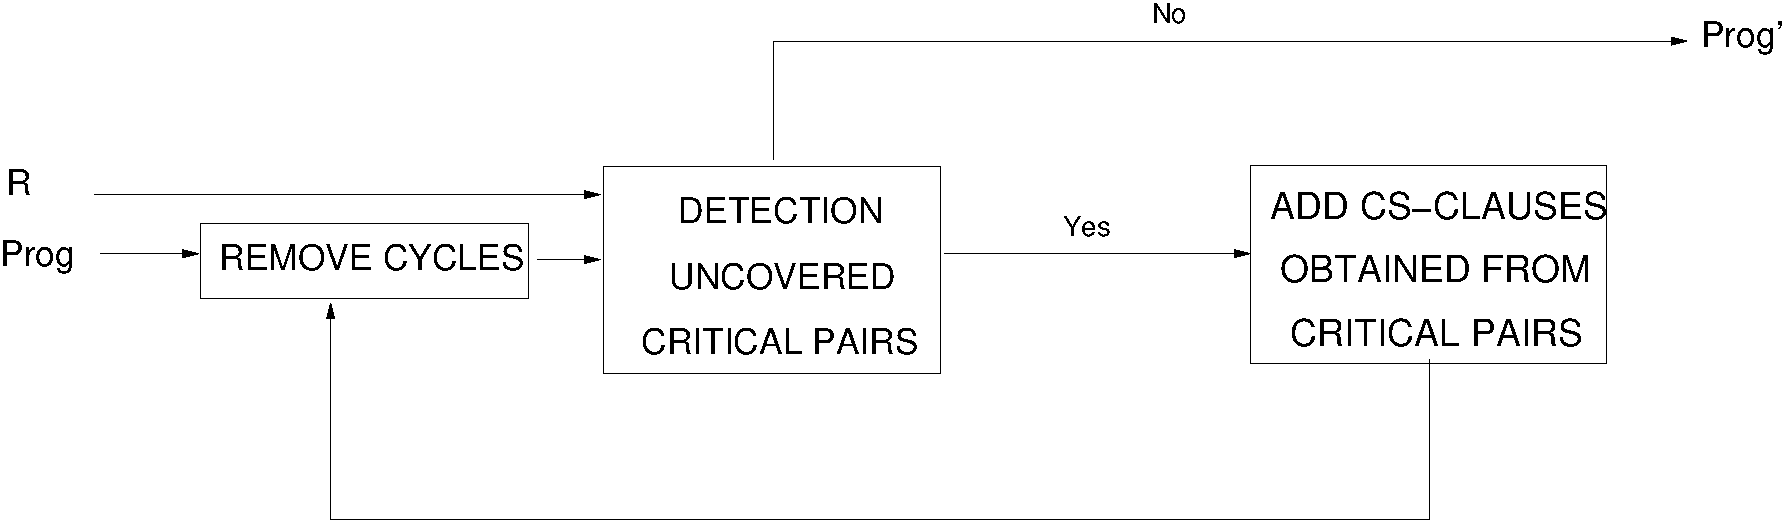
\includegraphics[width=\linewidth]{media/schema.pdf}\\
  \begin{itemize}[<+->]
  \item Le \csprogramme initial est
    \begin{itemize}
      \item non copiant
      \item normalisé
    \end{itemize}
    \vspace{\baselineskip}
  \item Le système de réécriture est
    \begin{itemize}
      \item linéaire
    \end{itemize}
  \end{itemize}
\end{frame}

\begin{frame}{Paires critiques}
  \begin{itemize}[<+->]
  \item ${\color<3>[rgb]{\focusrgb}l} \rightarrow r \in R$
  \item $P(..., {\color<3>[rgb]{\focusrgb}t_i}, ...) \leftarrow B \in Prog$
  \end{itemize}
  \begin{overprint}
    \onslide<3>
    $P(..., l, ...)$
    \onslide<4>
    $P(..., l, ...) $ \hfill $ \xrsquigarrow{~~~~~~~~~~~~~~~~~~~~~~~~~}^+_{[\sigma]} $ \hfill $ G$ avec $G$ plat \\
    \onslide<5>
    $P(..., l, ...) $ \hfill $ \xrsquigarrow{~~~~~~~~~~~~~~~~~~~~~~~~~}^+_{[\sigma]} $ \hfill $ G$ avec $G$ plat \\
    \begin{center}
      
\includegraphics[width=.8\linewidth]{media/CP1.pdf} \\
    \end{center}
    \onslide<6>
    $P(..., l, ...) $ \hfill $ \xrsquigarrow{~~~~~~~~~~~~~~~~~~~~~~~~~}^+_{[\sigma]} $ \hfill $ G$ avec $G$ plat \\
    \begin{center}
      
\includegraphics[width=.8\linewidth]{media/CP2.pdf} \\
    \end{center}
  \end{overprint}
  \onslide<5->
  $\sigma(P(..., r, ...)) \leftarrow G$ : paire critique
\end{frame}

\begin{frame}{Exemple}
  \begin{itemize}[<+->]
  \item $R$ : $\{{\color<3>[rgb]{\focusrgb}g(h(y))} \rightarrow f(y) \}$
  \item $Prog$ : $\{{\color<4>[rgb]{\focusrgb}{\color<3>[rgb]{\focusrgb}P(g(x))} \leftarrow Q(x)}; {\color<5>[rgb]{\focusrgb}Q(h(x)) \leftarrow Q'(x)}; Q'(a) \leftarrow \}$
  \end{itemize}
  \begin{overprint}
    \onslide<3>
    $P(g(h(y)))$
    \onslide<4>
    $P(g(h(y))) \xrsquigarrow{~~~~~~~~~~~~~~~~~~~~~~~~~} Q(h(y)) $
    \onslide<5>
    $P(g(h(y))) \xrsquigarrow{~~~~~~~~~~~~~~~~~~~~~~~~~} Q(h(y)) \xrsquigarrow{~~~~~~~~~~~~~~~~~~~~~~~~~} Q'(y)$ \\
    \onslide<6>
    $P(g(h(y)))$ \hfill $ \xrsquigarrow{~~~~~~~~~~~~~~~~~~~~~~~~~}^+_{[\sigma]} $ \hfill $ Q'(y)$ et $Q'(y)$ plat \\
    \onslide<7>
    $P(g(h(y)))$ \hfill $ \xrsquigarrow{~~~~~~~~~~~~~~~~~~~~~~~~~}^+_{[\sigma]} $ \hfill $ Q'(y)$ et $Q'(y)$ plat \\
    \begin{center}
      
\includegraphics[width=.8\linewidth]{media/CP1.pdf} \\
    \end{center}
    \onslide<8>
    $P(g(h(y)))$ \hfill $ \xrsquigarrow{~~~~~~~~~~~~~~~~~~~~~~~~~}^+_{[\sigma]} $ \hfill $ Q'(y)$ et $Q'(y)$ plat \\
    \begin{center}
      
\includegraphics[width=.8\linewidth]{media/CP2.pdf} \\
    \end{center}
  \end{overprint}
  \onslide<7->
  $\sigma(P(f(y))) \leftarrow Q'(y)$ : paire critique
\end{frame}

\begin{frame}{Le problème}
  \begin{itemize}[<+->]
  \item $Prog = \{ P(f(x,x)) \leftarrow Q(x).\,
    Q(a) \leftarrow .\,
    Q(b) \leftarrow .\}$
  \item $R = \{a \rightarrow b\}$ \\~

  \item Une paire critique : $Q(b) \leftarrow$
  \item Elle est convergente \\~

  \item $f(a, a) \in \mathcal{L}_{Prog}(P)$
  \item $f(a, a) \rightarrow_R f(b, a)$
  \item mais $f(b, a)$ et $f(a,b) \notin \mathcal{L}_{Prog}(P)$
  
  \end{itemize}
\end{frame}

\subsection{Descendants innermost}

\begin{frame}{Stratégie innermost}
  \begin{itemize}
  \item Restriction des réécritures
  \item Réécritures de sous-termes non réductibles
  \end{itemize}
  \begin{center}
    Figure à venir
  \end{center}
\end{frame}

\begin{frame}{Irréducibilité forte}
  \begin{Definition}[Irréducibilité forte]
    Soit $R$ un TRS.
    Un terme $t$ est {\em fortement irréducible} (par $R$) si
    pour tout $p \in \textit{PosNonVar}(t)$, pour tout $l \rightarrow r \in R$,
    $t|_p$ et $l$ ne sont pas unifiables.\\
    Une substitution $\theta$ est {\em fortement irréducible} si
    pour tout $x \in \mathcal{X}$, $\theta(x)$ est fortement irréducible.
  \end{Definition}
  \begin{itemize}
  \item \onslide<2-> $f(b) \rightarrow b$
  \item \onslide <3-> $t = f(x)$ : \onslide<4-> irréducible
  \item \onslide <5-> $\theta = (x/a)$ : \onslide <6-> est fortement irréducible
  \item \onslide <7-> $\theta(t) = f(a)$ : \onslide <8-> fortement irréducible
  \end{itemize}
\end{frame}

\begin{frame}{NC et SNC}
  \begin{Definition}
    Soit $A$ un atome ($A$ peut contenir des variables).\\
    L'étape $A \leadsto_{[H\leftarrow B,\sigma]} G$ est NC (resp.\ SNC) si
    pour tout $x \in Var^{mult}(H)$, $\sigma(x)$ est irréducible (resp.\ fortement irréducible) par $R$.\\
    Une dérivation est NC (resp.\ SNC) si toutes ses étapes le sont.
  \end{Definition}
  \begin{itemize}[<+->]
  \item Une clause non copiante est SNC \\~
    
  \item $P(g(x,x)) \leftarrow Q(x)$
  \item $R = \{h(a) \rightarrow b\}$ \\~

  \item $P(g(h(y),h(y))) \leadsto Q(h(y))$ : NC mais pas SNC
  \end{itemize}
\end{frame}

\begin{frame}{Clôture par réécriture innermost}
  \begin{alertblock}{Théorème [WRLA, 2016, Y. Boichut, V. Pelletier et P. Réty]}
    Soit $R$ un système de réécriture linéaire gauche.\\
    \pause
    Soit $Prog$ un \csprogramme normalisé et non copiant.\\
    \pause
    Soit $Prog' \supseteq Prog$ un \csprogramme \\
    \pause
    ~~~tel que toutes les paires critiques de $Prog$ sont convergentes\\
    ~~~par dérivations SNC dans $Prog'$.\\
    \pause
    Si un terme $t \in \mathcal{L}_{Prog}(P)$ et $t \rightarrow^*_R t'$ avec une stratégie innermost, alors $t' \in \mathcal L_{Prog'}(P)$.
  \end{alertblock}
\end{frame}


\subsection{Élimination des clauses copiantes}

\begin{frame}{Origine des clauses copiantes}
  \begin{itemize}[<+->]
  \item Les étapes de réécritures non couvertes proviennent des clauses copiantes
    \begin{itemize}
    \item Les clauses copiantes proviennent
      \begin{itemize}
      \item de clauses copiantes présentent dans le programme initial
      \item du système de réécriture non linéaire droit
      \end{itemize}
    \end{itemize}
    \vspace{\baselineskip}
  \item Solution
    \begin{itemize}
    \item une procédure pour transformer les clauses copiantes en non copiantes
    \end{itemize}
  \end{itemize}
\end{frame}

\begin{frame}{Exemple}
  \begin{itemize}[<+->]
  \item $Prog$ =
    \begin{itemize}
    \item $P(f(x,x)) \stackrel{1}{\leftarrow} Q(x)$
    \item \color<7>{focusColor}$Q(s(x)) \stackrel{2}{\leftarrow} Q(x)$
    \item \color<8>{focusColor}$Q(a) \stackrel{3}{\leftarrow} $
    \end{itemize}
    \vspace{\baselineskip}

  \item $uncopying(P(f(x,x)) \leftarrow Q(x))$
  \item $P(f(x,y)) \leftarrow Q^2(x, y)$
  \item $Q^2(s(x),s(y)) \leftarrow Q^2(x,y)$
  \item $Q^2(a,a) \leftarrow $ \\~

  \item Reconnaît le même langage
  \item Plus de clauses copiantes
  \end{itemize}
    
\end{frame}

\begin{frame}{Terminaison de l'élimination de clauses copiantes}
  \begin{itemize}[<+->]
  \item Ne termine pas dans le cas général
  \item $Prog$ =
    \begin{itemize}
    \item \color<7>{focusColor}$P(c(x,x)) \stackrel{1}{\leftarrow} P(x)$
    \item \color<8>{focusColor}$P(a) \stackrel{2}{\leftarrow} $
    \end{itemize}
    \vspace{\baselineskip}

  \item $uncopying(P(c(x,x)) \leftarrow P(x))$
  \item $P(c(x,y)) \leftarrow P^2(x, y)$
  \item \color<11>{focusColor}$P^2(c(x,x),c(y,y)) \leftarrow P^2(x,y)$
  \item \color<12>{focusColor}$P^2(a,a) \leftarrow $ \\~

  \item $uncopying(P^2(c(x,x), c(y,y)) \leftarrow P^2(x,y))$
  \item $P^2(c(x,x'), c(y,y')) \leftarrow P^4(x, x', y, y')$
  \item $P^4(c(x,x),c(x',x'),c(y,y),c(y',y')) \leftarrow P^4(x,x',y,y')$
  \item $P^4(a,a,a,a) \leftarrow $ \\~

  \item et ainsi de suite
  \end{itemize}
    
\end{frame}

\begin{frame}{Forcer la terminaison}
  \begin{itemize}[<+->]
  \item $UncopyingLimit = 2$ \\~

  \item $P^2(c(x,x'), c(y,y')) \leftarrow P^2(x, x'), P(y), P(y')$ \\~

  \item $\{ \vec{t}. \vec{t}. \vec{t'}. \vec{t''} \mid \vec{t},\vec{t'},\vec{t''} \in L(P) \} \subset L(P^4)$
  \end{itemize}
\end{frame}


\section{Transformation de systèmes de réécriture avec stratégie}

\begin{frame}{Stratégies de réécriture}
  \begin{itemize}
  \item Innermost
  \item context sensitive TRS
  \item prefix constrained TRS
  \item stratégie programmable
  \end{itemize}
\end{frame}

\begin{frame}{prefix constrained TRS}
  \begin{itemize}
  \item $L : l \rightarrow r$
  \item $Dir(\Sigma) = \{\langle f, i \rangle \mid f \in \Sigma, 1 \leq i \leq arity(f)\}$
  \item $L$ automate de mot construit sur $Dir(\Sigma)$
  \end{itemize}
  \begin{example}
    \begin{columns}
      \begin{column}{0.5\textwidth}
        \begin{itemize}
        \item $\Sigma = \{f^{\backslash 2}, g^{\backslash 2}, a^{\backslash 0}, b^{\backslash 0}\}$
        \item $R = \{L : a \rightarrow b\}$
        \item $L  = (\langle f,1 \rangle \cdot \langle g, 2 \rangle)^*$
        \item $t = f(g(a,a),a)$
        \end{itemize}
      \end{column}
      \begin{column}{0.5\textwidth}
        \begin{overprint}
          \onslide<1>
          \begin{tikzpicture}[level distance = 1cm]
            \node {$f$}
            child { node {$g$}
              child {node {$a$}}
              child {node {$a$}}}
            child {node {$a$}};
          \end{tikzpicture}
          \onslide<2>
          \begin{tikzpicture}[level distance = 1cm]
            \node {$f$}
            child {[color=red] node[color=black] {$g$}
              child {[color=black] node {$a$}}
              child {[color=red] node {$a$}}}
            child {node {$a$}};
          \end{tikzpicture}
          \onslide<3>
          \begin{tikzpicture}[level distance = 1cm]
            \node {$f$}
            child {[red] node[black] {$g$}
              child {[black] node {$a$}}
              child {[red] node {$b$}}}
            child {node {$a$}};
          \end{tikzpicture}
        \end{overprint}
      \end{column}
    \end{columns}
  \end{example}
\end{frame}

\begin{frame}{Transformation de TRS}
  \begin{itemize}
  \item $R' = R'_1 \cup R'_2 \cup R'_3 \cup R'_4$
  \item $R'_1 = \{top(j(x)) \rightarrow top(q_I(x)) \mid q_I \in Q_I\}$
  \item $R'_2= \{q(f(x_1,\ldots,x_n))\rightarrow \delta(x_1,\ldots,q'(x_i),\ldots,x_n) \mid \delta=(q, \langle f,i \rangle, q') \in \Delta\}$
  \item $R'_3= \{q_f(l_k) \rightarrow j(r_k) \mid q_f \in Q_f^k,\, (L_k : l_k \rightarrow r_k) \in R\}$
  \item $R'_4= \{\delta(x_1,\ldots,j(x_i),\ldots,x_n)\rightarrow j(f(x_1,\ldots,x_i,\ldots,x_n)) \mid \delta=(q, \langle f,i \rangle, q') \in \Delta\}$
  \end{itemize}
  \begin{alertblock}{Théorème : {\small[SCSS, 2017, N. Andrianarivelo, V. Pelletier et P. Réty]}}
    Soit $t \in T(\Sigma)$. On a $t \rightarrow^*_{R_{pc}} t'$ si et seulement si $top(j(t)) \rightarrow^*_{R'} top(j(t'))$.
  \end{alertblock}
  \begin{alertblock}{Théorème : {\small[SCSS, 2017, N. Andrianarivelo, V. Pelletier et P. Réty]}}
    Le pcTRS $R$ est terminant sur $\Sigma$ si et seulement si $R'$ est terminant sur $\Sigma'$.
  \end{alertblock}
\end{frame}

\begin{frame}{Exemple}
  \begin{columns}
    \begin{column}{0.5\textwidth}
      \begin{itemize}
      \item $\Sigma = \{f^{\backslash 2}, g^{\backslash 2}, a^{\backslash 0}, b^{\backslash 0}\}$
      \item $R=\{(\langle f,1 \rangle.\langle g,2 \rangle)^* : a\rightarrow b\}$
      \item $Dir(\Sigma)=\{\langle f,1 \rangle,\langle f,2 \rangle, \langle g,1 \rangle, \langle g,2 \rangle\}$
      \end{itemize}
    \end{column}
    \begin{column}{0.5\textwidth}
      \begin{tikzpicture}[shorten >=1pt,node distance=3cm,on grid,auto]
        \node[state,initial,accepting] (q) {$q$}; 
        \node[state] (q2) [right=of q] {$q'$};
      
        \path[->] 
        (q)   edge  [bend left]  node        {$(q,\langle f,1 \rangle, q')$} (q2)
        (q2)  edge  [bend left]  node        {$(q',\langle g,2 \rangle, q)$} (q);
      \end{tikzpicture}
    \end{column}
  \end{columns}
  \begin{columns}
    \begin{column}{0.6\textwidth}
      \begin{itemize}
      \item $R'_1= \{top(j(x)) \rightarrow top(q(x))\}$,
      \item $R'_2= \{q(f(x,y))\rightarrow \delta_1(q'(x),y),$\\$q'(g(x,y))\rightarrow \delta_2(x,q(y))\}$,
      \item $R'_3= \{q(a) \rightarrow j(b)\}$,
      \item $R'_4=\{\delta_1(j(x),y)\rightarrow j(f(x,y)),$\\$\delta_2(x,j(y))\rightarrow j(g(x,y))\}$.
      \end{itemize}
    \end{column}
    \begin{column}{0.4\textwidth}
      \begin{overprint}
        \onslide<1>
        \begin{tikzpicture}[level distance = 1cm]
          \node {$f$}
          child { node {$g$}
            child {node {$a$}}
            child {node {$a$}}}
          child {node {$a$}};
        \end{tikzpicture}
        \onslide<2>
        \begin{tikzpicture}[level distance = 1cm]
          \node {$top$}
          child { node {$j$}
            child{ node{$f$}
              child { node {$g$}
                child {node {$a$}}
                child {node {$a$}}}
              child {node {$a$}}}};
        \end{tikzpicture}
        \onslide<3>
        \begin{tikzpicture}[level distance = 1cm]
          \node {$top$}
          child { node {$q$}
            child{ node{$f$}
              child { node {$g$}
                child {node {$a$}}
                child {node {$a$}}}
              child {node {$a$}}}};
        \end{tikzpicture}
        \onslide<4>
        \begin{tikzpicture}[level distance = 1cm]
          \node {$top$}
          child { node {$\delta_1$}
            child{ node{$q'$}
              child { node {$g$}
                child {node {$a$}}
                child {node {$a$}}}
              child {node {$a$}}}};
        \end{tikzpicture}
        \onslide<5>
        \begin{tikzpicture}[level distance = 1cm]
          \node {$top$}
          child { node {$\delta_1$}
              child { node {$\delta_2$}
                child {node {$a$}}
                child {node {$q$}
                  child {node {$a$}}}}
              child {node {$a$}}};
        \end{tikzpicture}
        \onslide<6>
        \begin{tikzpicture}[level distance = 1cm]
          \node {$top$}
          child { node {$\delta_1$}
              child { node {$\delta_2$}
                child {node {$a$}}
                child {node {$j$}
                  child {node {$b$}}}}
              child {node {$a$}}};
        \end{tikzpicture}
        \onslide<7>
        \begin{tikzpicture}[level distance = 1cm]
          \node {$top$}
          child { node {$\delta_1$}
            child{ node{$j$}
              child { node {$g$}
                child {node {$a$}}
                child {node {$b$}}}
              child {node {$a$}}}};
        \end{tikzpicture}
        \onslide<8>
        \begin{tikzpicture}[level distance = 1cm]
          \node {$top$}
          child { node {$j$}
            child{ node{$f$}
              child { node {$g$}
                child {node {$a$}}
                child {node {$b$}}}
              child {node {$a$}}}};
        \end{tikzpicture}
      \end{overprint}
    \end{column}
  \end{columns}
\end{frame}

\section{Conclusion}

\begin{frame}{Conclusion}
  \begin{itemize}[<+->]
  \item Calcul de sur-approximations non régulières
    \begin{itemize}
    \item Descendants innermost
    \item Élimination de clauses copiantes
    \end{itemize}
  \item Transformation de pcTRS
  \item Transformation d'un programme logique en \csprogramme avec sur-approximation
  \end{itemize}
\end{frame}

\begin{frame}{Perspectives}
  \begin{itemize}[<+->]
  \item Calcul de sur-approximations non régulières
    \begin{itemize}
    \item Améliorer la précision des approximations
    \item Développer des Heuristiques
    \item Porter les résultats existants sur les réguliers
    \end{itemize}
  \item Transformation de pcTRS
    \begin{itemize}
      \item Explorer d'autres stratégies
    \end{itemize}
  \item Transformation d'un programme logique en \csprogramme avec sur-approximation
    \begin{itemize}
    \item Améliorer la précision des approximations
    \end{itemize}
  \end{itemize}
\end{frame}

\begin{frame}{Remarques et questions}
  \begin{center}
    Merci de votre attention
  \end{center}
\end{frame}

\end{document}